\documentclass[tikz,border=5mm]{standalone}
\usetikzlibrary{
arrows, decorations.pathmorphing, 
backgrounds, positioning, 
fit, petri
}
\begin{document}

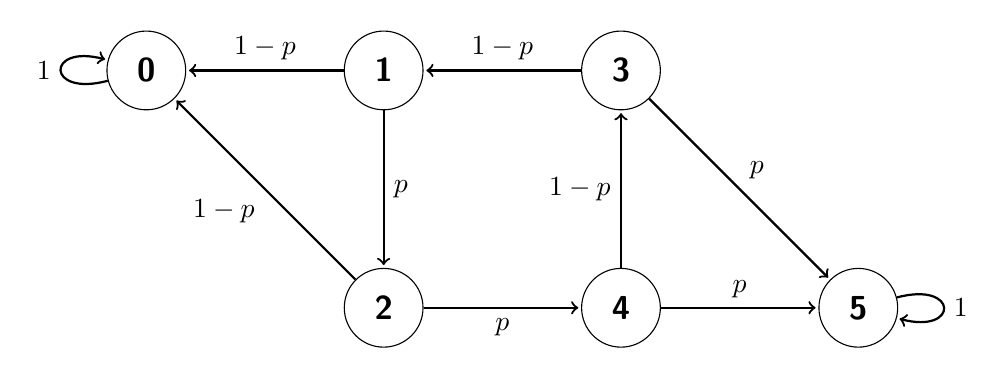
\begin{tikzpicture}[
	state/.style={
	minimum size=1cm, 
	circle,draw,font=\sffamily\large\bfseries
	}, 
	node distance = 20mm
]

% NODES
\node [state] 	(0)      				{0};
\node [state] 	(1) [right=of 0]		{1};
\node [state] 	(2) [below=of 1]		{2};
\node [state] 	(3) [right=of 1]		{3};
\node [state]	(4) [right=of 2]		{4};
\node [state]	(5) [right=of 4]		{5};
   
% PATHS     
\path [thick,shorten >= 1pt,auto]
(0) edge [->, loop left]  node {1} (0)
(5) edge [->, loop right]  node {1} (5)
(1) edge [->, above] node {$1 - p$} (0)
(2) edge [->] node {$1 - p$} (0)
(1) edge [->] node {$p$} (2)
(4) edge [->] node {$1 - p$} (3)
(3) edge [->] node {$p$} (5)
(4) edge [->] node {$p$} (5)
(3) edge [->, above] node {$1 - p$} (1)
(2) edge [->, below] node {$p$} (4);

\end{tikzpicture}


\end{document}